\chapter{Datasets}
\label{chap:data}

% TODO was it really mentioned
As mentioned, the primary dataset, usage-wise and inspiration-wise, was the FEVER dataset \citep{fever}.
Deriving from \cite{fever} methods, we \citep{ullrich} were able to create our own FEVER-like database using Czech News Agency's infobank.

\section{FEVER Dataset}

\textbf{F}act \textbf{E}xtraction and \textbf{Ver}ification \citep{fever} dataset is a large-scale dataset based on Wikipedia articles.
The dataset was created by extracting sentences (claims) from the English Wikipedia articles and classifying them by human annotators as Supported, Refuted, or NotEnoughInfo.
If the claim is verifiable (Supported, Refuted), then the evidence, either single or multiple paragraphs or even articles proving or disproving the claim, is also recorded.
The complete FEVER contains 185,445 annotated claims generated using 50,000 popular articles.

The creation consisted of two steps. The sentences were first manually extracted from popular Wikipedia articles.
Only the first paragraphs, usually containing the summary, were used for this step. 
Then, to create a more diverse set of claims, the annotators had the option of producing new claims by mutating the existing ones in various ways (generalizing, specification, entity substitution, non-trivial negating, and rephrasing).
The negation used has to be non-trivial because simple negative words and phrases like ``no'' and ``it is not true that'' can be leveraged by the later steps of the fact-checking pipeline to immediately classify claims as Refuted instead of trying to understand the text.

More complex claims were created by providing related Wikipedia articles (articles hyperlinked from the original article) as another source of information while mutating the claim.

In the second step - annotation - the annotators were asked to label the generated claims and provide suggested evidence when needed.
The whole process was streamlined to not spend longer than five minutes on a single claim throughout all stages.

The quality of the dataset was throughoutly tested in the paper.
One of the methods for improving the dataset was annotating the generated claim by multiple people to reduce mislabeling.

\subsection{FEVER CS}

For use in baseline training and pre-training, we localized the original FEVER dataset into the Czech language. 
The localization consisted of translating the original claims using a translation service and mapping the English Wikipedia knowledge base used by FEVER to available Czech Wikipedia articles while removing claims with missing Czech evidence.
The process is in-depth described by \citet[Chapter 3]{ullrich}.

\begin{table}[h!]
    \centering
    \begin{tabular}{c || c c c || c c c}
        \multirow{2}{0.8cm}{Split} & \multicolumn{3}{c||}{FEVER CS} & \multicolumn{3}{c}{FEVER EN} \\
        & Supported & Refuted & NEI & Supported & Refuted & NEI\\
        \hline
        train & 53,542 & 18,149 & 35,639 & 80,035 & 29,775 & 35,639\\
        dev & 3,333 & 3,333 & 3,333 & 6,666 & 6,666 & 6,666 \\
        test & 3,333 & 3,333 & 3,333 & 6,666 & 6,666 & 6,666
    \end{tabular}
\caption[Fever CS Label Distribution]{Label distribution of the resulting FEVER CS.}
\end{table}

Because of the large-scale usage of machine translation without the means for robust evaluation and the lack of one-to-one correspondence between Czech and English Wikipedia articles, this dataset serves only as a baseline to verify the robustness of our models on a larger scale, primarily for the document retrieval part of the pipeline.

\begin{figure}[h!]
    \begin{framed}
    \begin{verbatim}
    {
      "id": 120449,
      "verifiable": "VERIFIABLE",
      "label": "SUPPORTS",
      "claim": "Venuše se nazývá 'sesterskou planetou' Země.",
      "evidence": [
        [
          [
            141476,
            156671,
            "Venuše (planeta)",
            8,
            "Venus"
          ]
        ]
      ],
      "claim_en": "Venus is called the \"sister planet\" of Earth."
    }\end{verbatim}
    \vspace{-0.4cm}
    \end{framed}
    \caption[FEVER CS Data Example]{FEVER CS data example, containing one evidence set refering to the Venus Wikipedia page.}
    \label{fig:fevercs_example}
\end{figure}

\section{\CTK}
% nomenclature

The basis for this dataset is the collection of Czech news articles provided in collaboration with the Czech News Agency. 
Inspired by \cite{fever} and \cite{danish_fever}, our colleague \cite{ullrich} created a Czech version of the claim extracting and labeling software tool\footnote{available at \url{https://fcheck.fel.cvut.cz/}} running over the ČTK infobank's articles. 
%TODO insert image
It was designed to be used by layman annotators, who were students of our partner - the Faculty of Social Sciences at Charles University.

\begin{table}[h!]
\centering
\begin{tabular}{c || c c c}
    Split & Supported & Refuted & NotEnoughInfo \\
    \hline
    train & 1132 & 519 & 473 \\
    dev & 100 & 100 & 100 \\
    test & 200 & 200 & 200
\end{tabular}
\caption[\CTK{} Dataset Label Distribution]{Label distribution of the resulting \CTK{} v2.1 dataset.}
\end{table}

The dataset creation consisted of two harvests. 
After reviewing the results of the first one, we were able to rewrite instructions in the tool to guide the annotators to create higher-quality mutations and labels with fewer conflicts.
The second harvest concluded with $\approx$ 3,500 labeled claims, with more than half being labeled two or more times. %TODO cite webpage
As of writing, this figure is not final as the dataset needs to be manually cleaned and have conflicts resolved. 

\begin{figure}[h!]
    \begin{framed}
    \begin{verbatim}
    {
      "id": 2143,
      "label": "REFUTES",
      "claim": "Kocianovo kvarteto nikdy nezískalo žádné ocenění.",
      "evidence": [
        [
          "T200706010229101_1"
        ]
      ],
      "source": "T200706010229101_1"
    }\end{verbatim}
    \vspace{-0.4cm}
    \end{framed}
    \caption[\CTK{} Dataset Example]{\CTK{} data example, containing one evidence set refering to the first paragraph of the \CTK{} infobank article with the id \texttt{T200706010229101}.}
    \label{fig:ctk_example}
\end{figure}

\begin{figure}[h!]
    \begin{framed}
        Paříž/Praha 2. června (ČTK) - Za vynikající kompletní nahrávku kvartetů Paula Hindemitha pro francouzskou firmu Harmonia Mundi obdrželo 3. června 1997 české Kocianovo kvarteto Velkou cenu francouzské Akademie Charlese Crose.
    \end{framed}
    \caption[\CTK{} Infobank Example]{\CTK{} infobank entry corresponging to the evidence id in Figure \ref{fig:ctk_example}.}
\end{figure}

\begin{figure}[h!]
  %\makebox[\textwidth][c]{{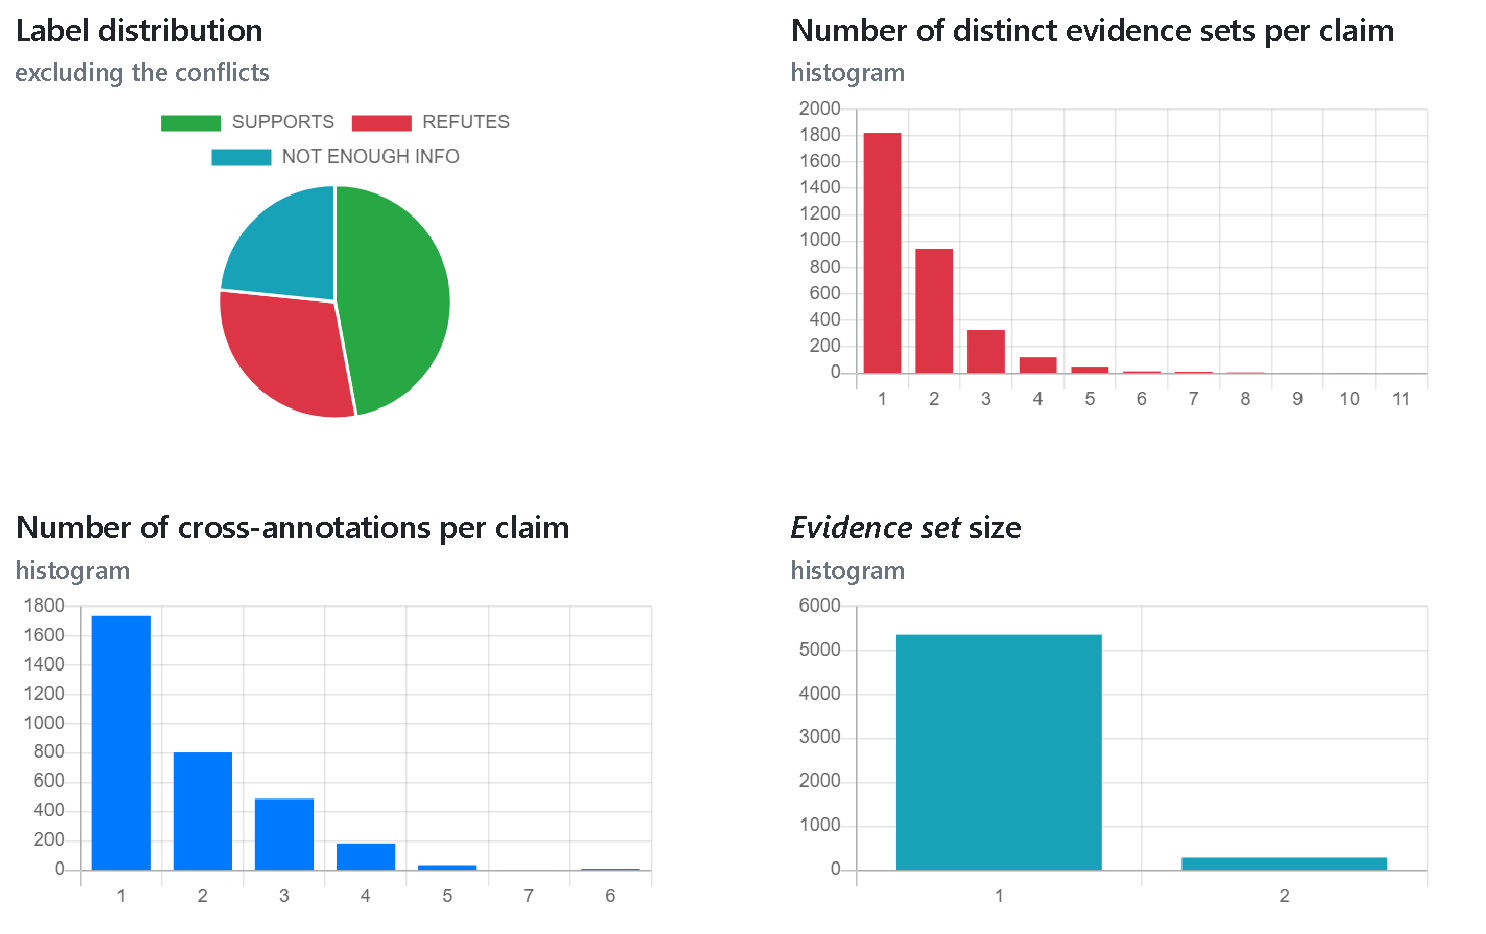
\includegraphics[width=16cm]{dashboard.pdf}}}
  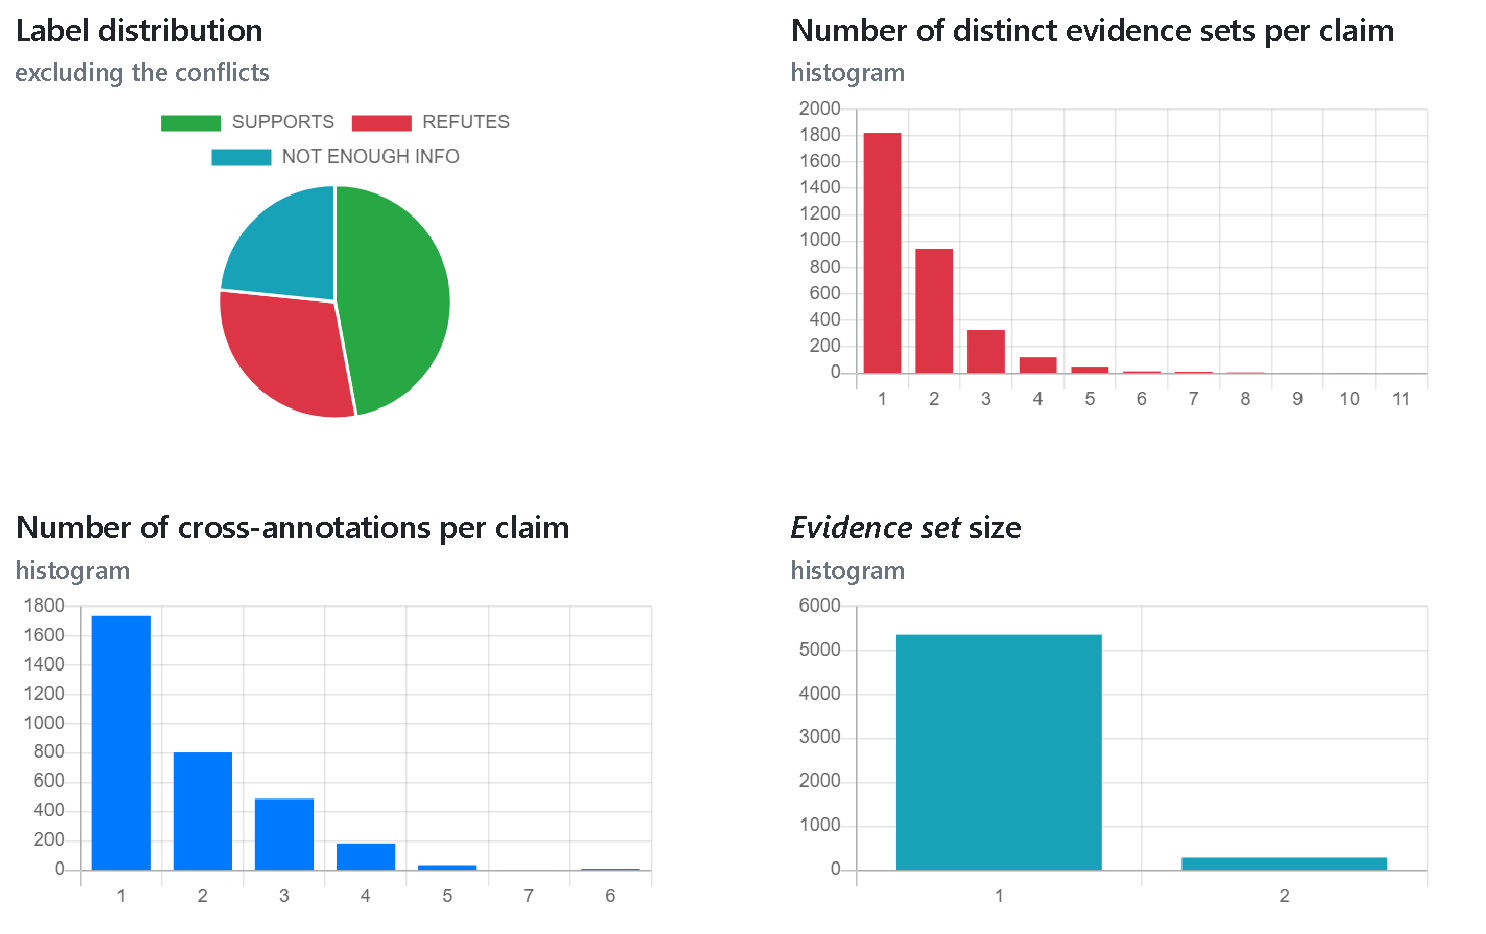
\includegraphics[width=\textwidth]{dashboard.pdf}
  \caption[Visualizations of Properties of the Collected Dataset]{Visualizations of various properties of the collected \CTK{} dataset. Figure reprinted from \citet{ullrich}.}
  \label{fig:dashboard}
  \end{figure}

\section{Data Quality}

The claim mutation in FEVER and \CTK{} datasets can be a source of unintentional cues, which the model can use to "guess" the label without understanding the claim.
For example, \citet{fever} pointed out that their annotators had difficulties negating the claims beyond trivial negations.

\citet{rypar} conducted a series of evaluations on the \CTK{} and FEVER CS datasets using dataset-weighted cue information (DCI), and cue productivity and coverage \citep{niven-probing}, inpsired by \citet{derczynski-etal-2020-maintaining}. 
The results concluded that the original FEVER dataset contained simple negative clues, which were also present in FEVER CS, although with limited impact only. No significant bias was confirmed, but the current size of the \CTK{} dataset allows for thematic clusters which impact the dataset more than they should. 

\subsection{Data Leakage}

As pointed out by \citet{ullrich}, the original FEVER dataset CONTAINS a not addressed quality -- at least 80 \% of verifiable dev claims share an evidence-set document with some train claim. The effects of this "leakage" are unknown and call for further research.